% ACCESS-AIS3 internal status talk (~15 min, ACCESS-NRI team). Numbers from
% docs/post_inversion_pipeline_worklog.md (sections cited in the notes).
% Build: pdflatex ais3_internal.tex (twice). Speaker notes: uncomment the show notes line below.
\documentclass[aspectratio=169,10pt]{beamer}
% \setbeameroption{show notes on second screen=right}

\usepackage[T1]{fontenc}
\usepackage[utf8]{inputenc}
\usepackage{tgheros}
\renewcommand{\familydefault}{\sfdefault}
\usepackage{graphicx}
\usepackage{xcolor}
\usepackage{colortbl}
\usepackage{booktabs}
\usepackage{ragged2e}
\AtBeginDocument{\RaggedRight}
\graphicspath{{figs/}}

% ---- palette (as the overview deck)
\definecolor{navy}{HTML}{14213D}
\definecolor{paper}{HTML}{FBFBF8}
\definecolor{paper2}{HTML}{EEF1EF}
\definecolor{ink}{HTML}{1F2A37}
\definecolor{muted}{HTML}{3D4A5C}
\definecolor{faint}{HTML}{5A6676}
\definecolor{accent}{HTML}{B4410E}
\definecolor{blue}{HTML}{1D5FA8}
\definecolor{green}{HTML}{0F7A5C}
\definecolor{sand}{HTML}{F4A261}
\definecolor{mist}{HTML}{B8C4D6}
\definecolor{cream}{HTML}{F3F1EA}

\newcommand{\serif}{\fontfamily{qpl}\selectfont}

\setbeamertemplate{navigation symbols}{}
\setbeamercolor{background canvas}{bg=paper}
\setbeamercolor{normal text}{fg=ink}
\setbeamercolor{itemize item}{fg=accent}
\setbeamertemplate{itemize item}{\small$\bullet$}
\setbeamertemplate{itemize subitem}{\scriptsize--}
\setbeamersize{text margin left=10mm, text margin right=10mm}
\setbeamertemplate{frametitle}{%
  \vspace*{5mm}%
  {\scriptsize\bfseries\color{accent}\MakeUppercase{\insertframesubtitle}}\par\vspace{1mm}%
  {\serif\Large\bfseries\color{navy}\insertframetitle}\par}
\setbeamertemplate{footline}{%
  \hbox to \paperwidth{\hspace{10mm}{\tiny\color{faint}\insertshortsource}\hfill
  {\tiny\color{faint}\insertframenumber}\hspace{10mm}}\vspace{4mm}}
\makeatletter
\newcommand{\insertshortsource}{\beamer@shortsource}
\newcommand{\source}[1]{\gdef\beamer@shortsource{#1}}
\gdef\beamer@shortsource{}
\makeatother
\newcommand{\nosource}{\source{}}

% status tags
\newcommand{\done}{{\bfseries\color{green}done}}
\newcommand{\running}{{\bfseries\color{blue}running}}
\newcommand{\open}{{\bfseries\color{accent}open}}
\newcommand{\hl}[1]{{\bfseries\color{accent}#1}}

\begin{document}

% ============================================================ title
{\setbeamercolor{background canvas}{bg=navy}
\setbeamertemplate{footline}{}
\begin{frame}
\vfill
{\scriptsize\bfseries\color{sand}INTERNAL \textperiodcentered{} STATUS UPDATE}\par\vspace{4mm}
{\serif\fontsize{36}{40}\selectfont\bfseries\color{cream}ACCESS-AIS3}\par\vspace{4mm}
{\large\color{mist}Pipeline, projections to 2300, LARMIP diagnosis, HO findings, and decisions we need}
\vfill
{\small\color{mist}Justin Hew \textperiodcentered{} ACCESS-NRI \textperiodcentered{} 6 November 2026}
\vspace{6mm}
\end{frame}}

% ============================================================ status
\nosource
\begin{frame}{Where things stand}
\framesubtitle{Status at a glance}
\vspace{1mm}\footnotesize
\begin{tabular}{@{}p{0.27\linewidth}p{0.1\linewidth}p{0.56\linewidth}@{}}
\toprule
\textbf{Component} & \textbf{State} & \textbf{Detail}\\
\midrule
SSA chain to 2019 & \done & Budd $p=q=1$; melt $\gamma_0=300$ + per-basin $\Delta T$; historical 1995--2019\\
SSA projections to 2300 & \done & SSP1-2.6/5-8.5 (CESM2, MRI), ssp370 $\times$7 GCMs to 2100, attribution, high melt\\
ISMIP7 shelf collapse & \done & SSP5-8.5 CESM2: +526 vs +211 mm at 2300\\
LARMIP-3 & \done & submitted 23 Oct; two questions with Anders \open\\
HO chain (D2 + relaxfix) & \done & historical rerun from relaxed start; HO vs SSA to 2100 within 5\%\\
HO projections to 2300 & \running & ctrl at 2180, ssp585 at 2230; $\sim$10 Nov (ssp585), $\sim$13 Nov (ctrl)\\
HO velocity pins & \open & 8.4\% of grounded ice held at obs speed; can't be removed\\
Paper & \open & GMD model description proposed; scope to agree\\
\bottomrule
\end{tabular}
\end{frame}

% ============================================================ pipeline
\begin{frame}{Two tracks share mesh and forcing; SSA is production}
\framesubtitle{Pipeline}
\vspace{2mm}\small
\begin{columns}[T]
\column{0.48\textwidth}
{\serif\large\bfseries\color{navy}SSA} \hfill {\scriptsize\color{faint}\texttt{config/ais\_0.1\_SSA.py}}
\begin{itemize}
\item Inversion: Budd $p=q=1$, 1.59 M vertices
\item Melt: ISMIP6-style, $\gamma_0=300$, refit $\Delta T$ per basin
\item Starts from the inverted (unrelaxed) geometry, by design
\item Historical 1995--2019, then anomaly-forced chunks to 2300
\end{itemize}
\column{0.48\textwidth}
{\serif\large\bfseries\color{navy}HO (Blatter--Pattyn)} \hfill {\scriptsize\color{faint}\texttt{config/ais\_0.1.py}}
\begin{itemize}
\item 15 layers, 23.8 M vertices; thermal steady state
\item Friction re-inversion paused after chunk 3 (RMSE 94--99 m/yr)
\item D2 rheology: per-column rescale to SSA's deformation-weighted $B$ (HO flowed 10--15\% fast)
\item Relaxation end state now propagated (relaxfix)
\item Velocity pins from the Schoof subdomain carried into transients
\end{itemize}
\end{columns}
\note{Worklog sections 1, 4z, 5a-5d, 5e. The SSA unrelaxed start is deliberate (only HO propagates its relaxation). D2: grounded columns match the deformation-weighted column B, w = (1 - sigma)^(n+1); floating columns the plain mean.}
\end{frame}

% ============================================================ historical
\source{Grounded ice with CPOM coverage every year (7.56 M km$^2$), area-weighted. Worklog 4r--4t, 5b, 6.13.}
\begin{frame}{Historical runs track CPOM once the start-up transient is over}
\framesubtitle{Evaluation, 1996--2019}
\begin{columns}[c]
\column{0.58\textwidth}\centering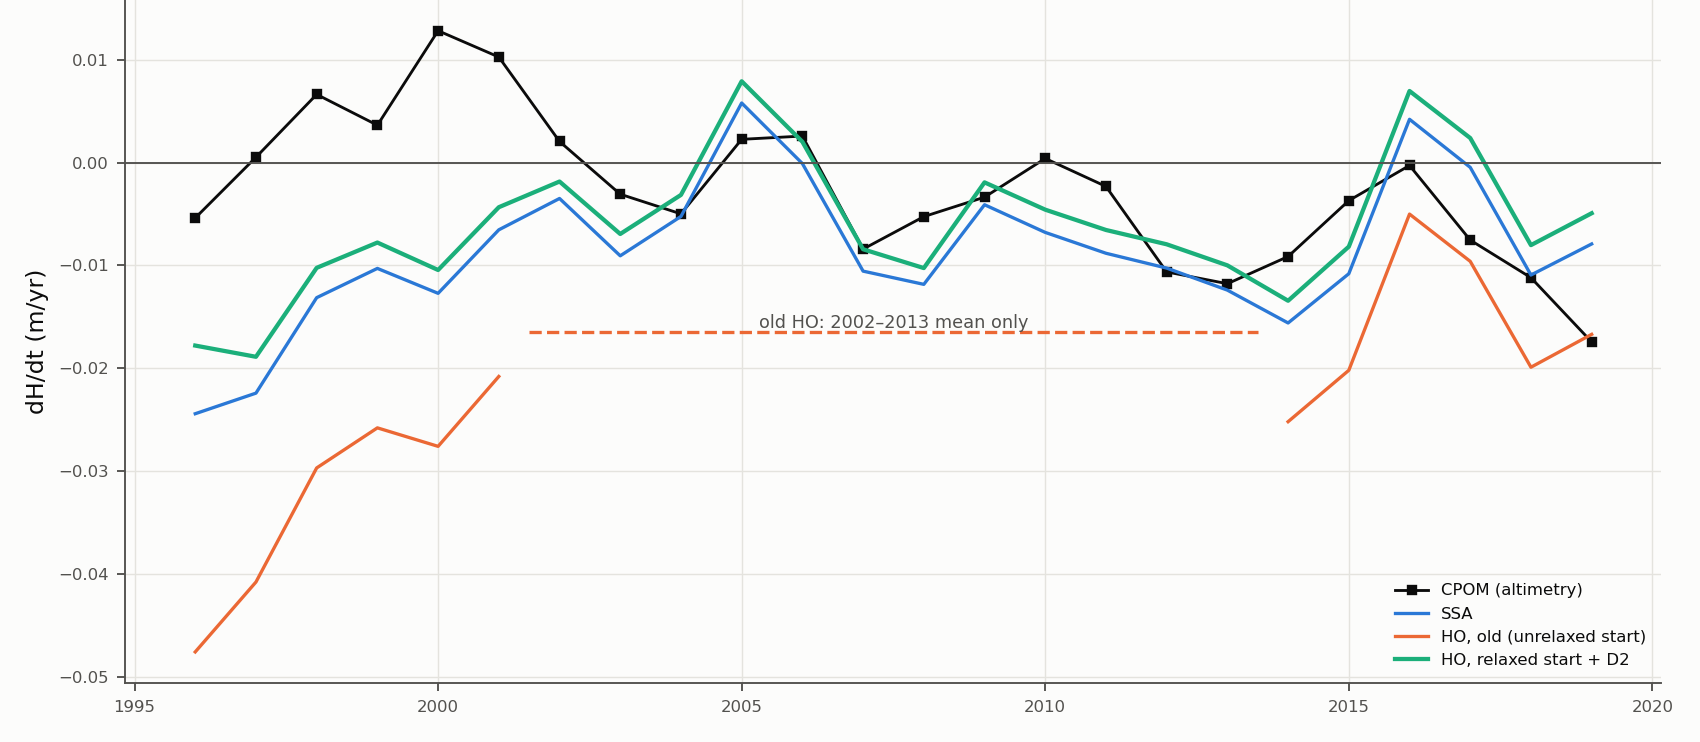
\includegraphics[width=\linewidth]{historical.png}
\column{0.38\textwidth}\small
\begin{itemize}
\item Interannual swings are SMB-driven and match after $\sim$2004
\item First $\sim$6 years too negative: start-up transient
\item Relaxed HO + D2 (green) fixes the old HO's large thinning bias (orange)
\item Misses the West Antarctic dynamic thinning (basin 9)
\item Don't quote the production ``RMSE'' (SSA 1.40, HO 1.77 m/yr): spatial, 2019 slice only
\end{itemize}
\end{columns}
\end{frame}

% ============================================================ campaign
\source{Sea level minus control, mm, + = rise; ISMIP-convention VAF (\texttt{models/proj\_ssa\_sle\_series.csv}). Worklog 6.11.}
\begin{frame}{SSA campaign: SMB-dominated, with a GCM-specific late reversal}
\framesubtitle{Projections}
\vspace{1mm}\small
\begin{columns}[T]
\column{0.58\textwidth}
\begin{tabular}{@{}lrrrrr@{}}
\toprule
\textbf{Run} & \textbf{2100} & \textbf{2150} & \textbf{2200} & \textbf{2250} & \textbf{2300}\\
\midrule
ssp126 CESM2 & $-$43 & $-$82 & $-$121 & $-$167 & $-$213\\
ssp585 CESM2 & $-$73 & $-$143 & $-$148 & $-$19 & \hl{+211}\\
\quad high melt & $-$59 & $-$97 & $-$62 & +86 & +313\\
\quad ocean only & +1 & +4 & +10 & +19 & +31\\
\quad SMB only & $-$74 & $-$147 & $-$156 & $-$33 & \\
\quad collapse & & & & & \hl{+526}\\
ssp126 MRI & $-$18 & $-$37 & $-$62 & $-$91 & $-$124\\
ssp585 MRI & $-$42 & $-$80 & $-$80 & $-$60 & $-$39\\
\bottomrule
\end{tabular}
\column{0.38\textwidth}
\begin{itemize}
\item Reversal is SMB-driven and near-additive; much weaker with MRI
\item ssp370 at 2100 across 7 GCMs: $-$34 (MPI) to $-$64 (ACCESS-CM2)
\item Ocean-only is small partly by calibration: J3 shows $\gamma_0=300$ gives $\sim$4\% of ocean models' warming response
\item High melt ($\gamma_0=15000$): +100 mm by 2300
\end{itemize}
\end{columns}
\note{The SMB-only 2300 value was still running when the table in 6.11 was written; fill in from proj_ssa_sle_series.csv if needed. J3 is from 6.1.}
\end{frame}

% ============================================================ projection figure
\source{ACCESS-AIS3 (SSA), minus control. (a) CESM2-WACCM scenarios and melt; (b) SSP5-8.5 attribution; (c) ssp370, seven GCMs.}
\begin{frame}{The same story in the figures}
\framesubtitle{Projections}
\vspace{3mm}
\centering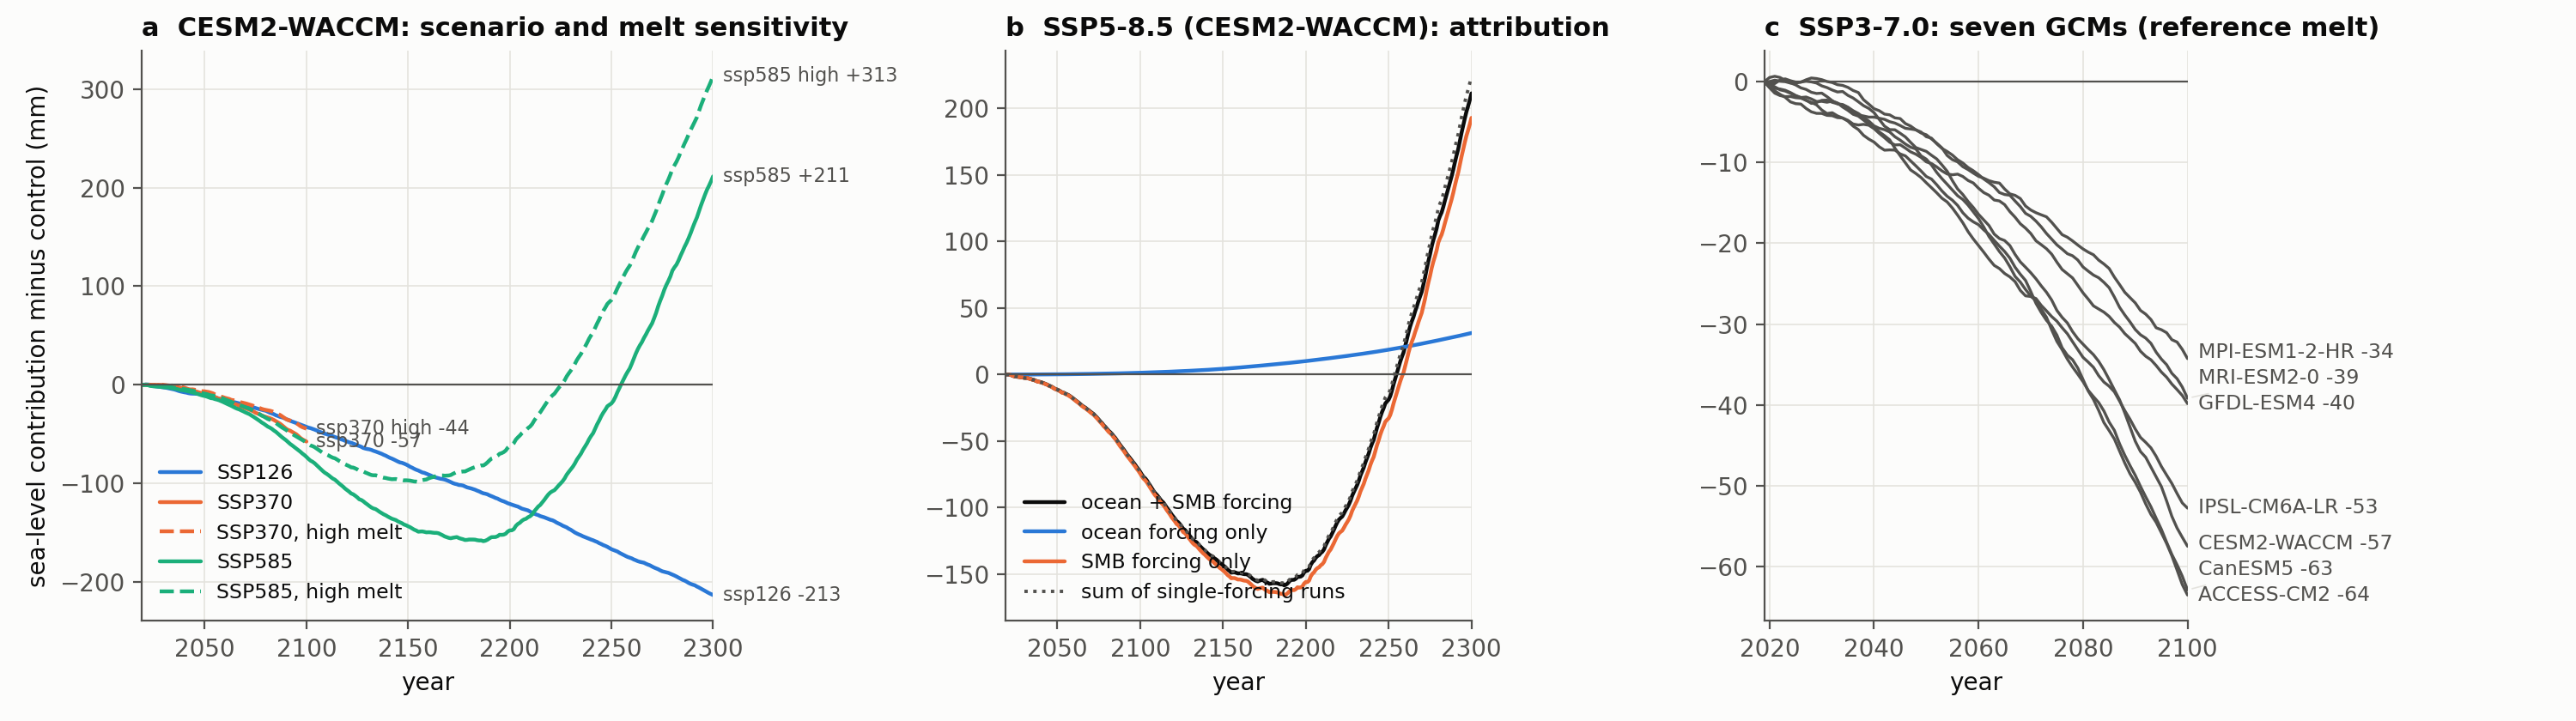
\includegraphics[width=\linewidth]{projections_ssa.png}
\end{frame}

% ============================================================ collapse
\source{SSP5-8.5 CESM2-WACCM; ISMIP7 fracture path C, mask v2.1. Worklog 6.12, 6.15, 6.18.}
\begin{frame}{Collapse adds 315 mm by 2300; the implementation needed several fixes}
\framesubtitle{ISMIP7 shelf collapse}
\vspace{1mm}
\centering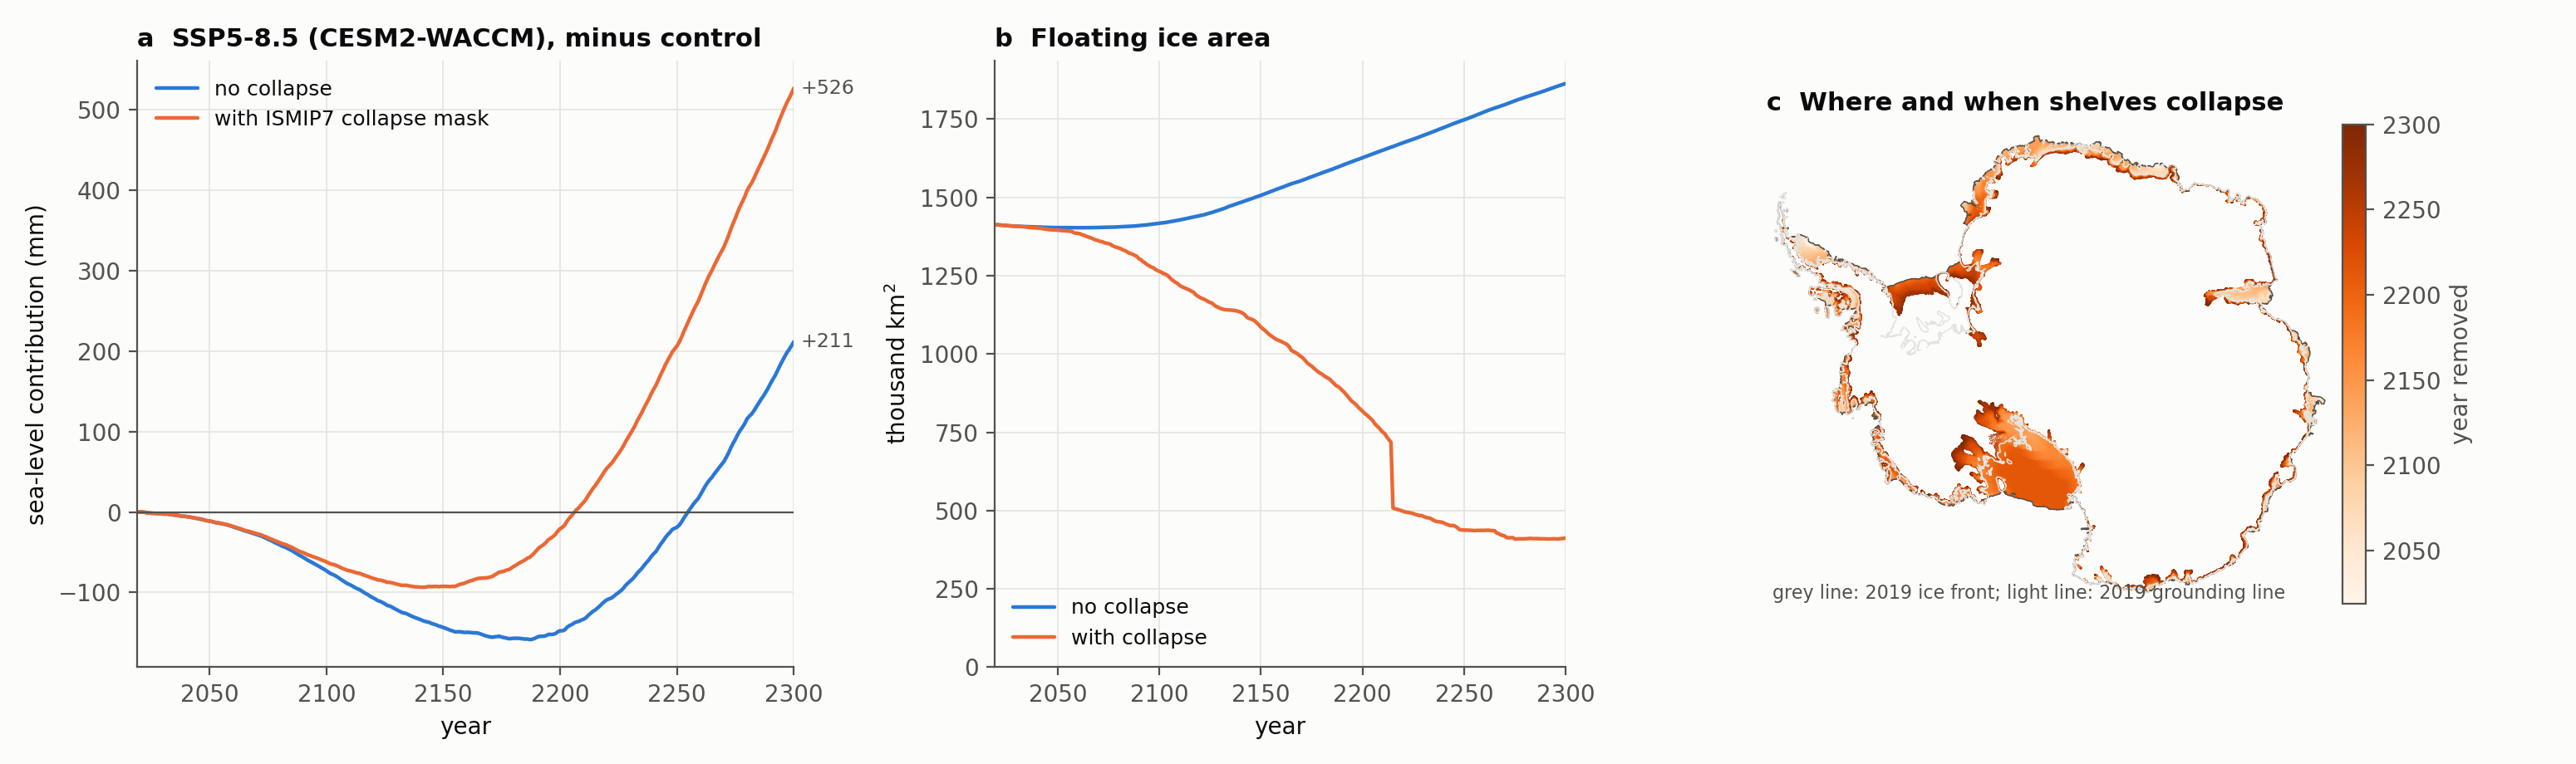
\includegraphics[width=0.74\linewidth]{collapse.png}\par\vspace{1mm}
\scriptsize
\begin{columns}[T]
\column{0.48\textwidth}
\begin{itemize}
\item Each 1 Jan: masked floating ice gets ice\_levelset $=+1$, $H=1$ m, flotation state
\item Every unanchored piece removed each year (anchor = fully grounded element with $C>0$); fixed the 2089 NaN
\end{itemize}
\column{0.48\textwidth}
\begin{itemize}
\item Yearly sub-solves at mask changes; watched solve with one retry
\item Residue threshold 1e-2 for collapse runs (1e-3 elsewhere) \open
\item Ross: most of the shelf removed in 2214
\end{itemize}
\end{columns}
\note{Earlier attempts: melt-anomaly collapse blew up; rigid-body NaN fixed by requiring C > 0 and edge connectivity; base = bed on grounded ice fixed by giving removed vertices the flotation state of 1 m ice; 2089 failure traced to unanchored pieces.}
\end{frame}

% ============================================================ larmip
\source{LARMIP 8 m/yr step, AIS3 sectors minus control vs LARMIP-2 (upper 10\% clipped). Worklog 6.14--6.18.}
\begin{frame}{LARMIP: AIS3 sits at the bottom of the LARMIP-2 spread}
\framesubtitle{Sensitivity}
\vspace{1mm}
\centering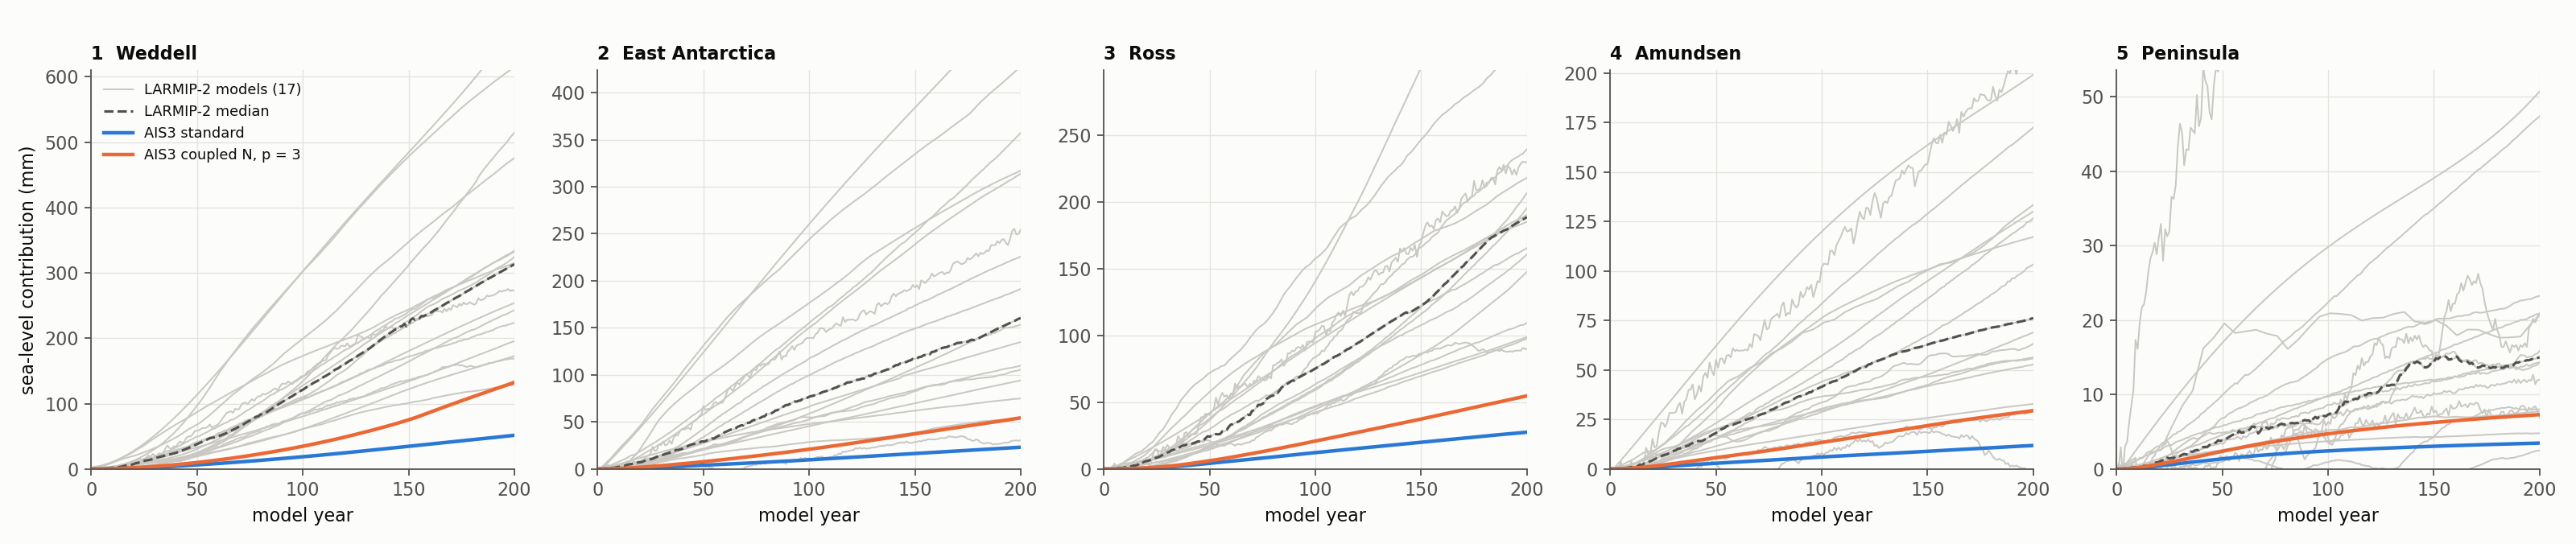
\includegraphics[width=0.9\linewidth]{larmip.png}\par\vspace{1mm}
\small
\begin{columns}[T]
\column{0.48\textwidth}
\begin{itemize}
\item Standard set 4--7$\times$ below the LARMIP-2 median at year 200
\item Shelves thin almost completely, but grounded speed-up only $\times$1.05--1.2
\end{itemize}
\column{0.48\textwidth}
\begin{itemize}
\item Measured: flotation $N$ $\times$1.5 (y50); $p=3$ $\sim\times$2 (y200); melt at GL $\times$1.34 (y30)
\item coupledN\_p3 (submitted main set) still 2--3.5$\times$ below
\item Left: high inverted drag near GL, resolution, SSA
\end{itemize}
\end{columns}
\end{frame}

% ============================================================ HO vs SSA
\source{ISMIP-convention VAF, mm, minus control. HO beyond 2100 from the running extension.}
\begin{frame}{HO agrees with SSA to 2100; after that its ctrl drift pulls the difference apart}
\framesubtitle{HO vs SSA}
\vspace{2mm}\small
\begin{columns}[T]
\column{0.5\textwidth}
\begin{tabular}{@{}lrrrr@{}}
\toprule
& \multicolumn{2}{c}{\textbf{ssp585 $-$ ctrl}} & \multicolumn{2}{c}{\textbf{ctrl drift}}\\
\textbf{Year} & HO & SSA & HO & SSA\\
\midrule
2100 & $-$70 & $-$73 & $-$65 & $-$41\\
2130 & $-$108 & $-$121 & $-$89 & $-$54\\
2150 & $-$120 & $-$143 & $-$105 & $-$62\\
2180 & $-$117 & $-$157 & $-$130 & $-$74\\
\bottomrule
\end{tabular}
\column{0.46\textwidth}
\begin{itemize}
\item ssp585 alone tracks SSA (HO 15--20 mm lower); both bottom out $\sim$2190 and rise $\sim$55 mm by 2230
\item HO ctrl gains 8 mm/decade vs SSA 4: the cause of the gap
\item Hypothesis: pinned columns can't speed up to evacuate SMB gain (untested)
\item Use HO for timing of the turnaround, not the post-2100 number
\end{itemize}
\end{columns}
\end{frame}

% ============================================================ pins
\source{\texttt{models/ho\_pins\_by\_basin.csv}, \texttt{models/ho\_unpin\_test.npz}. Worklog 6.20--6.21.}
\begin{frame}{HO holds velocity at observed values on 8\% of grounded ice, 64\% of Ross GL flux}
\framesubtitle{HO velocity pins}
\begin{columns}[T]
\column{0.34\textwidth}\centering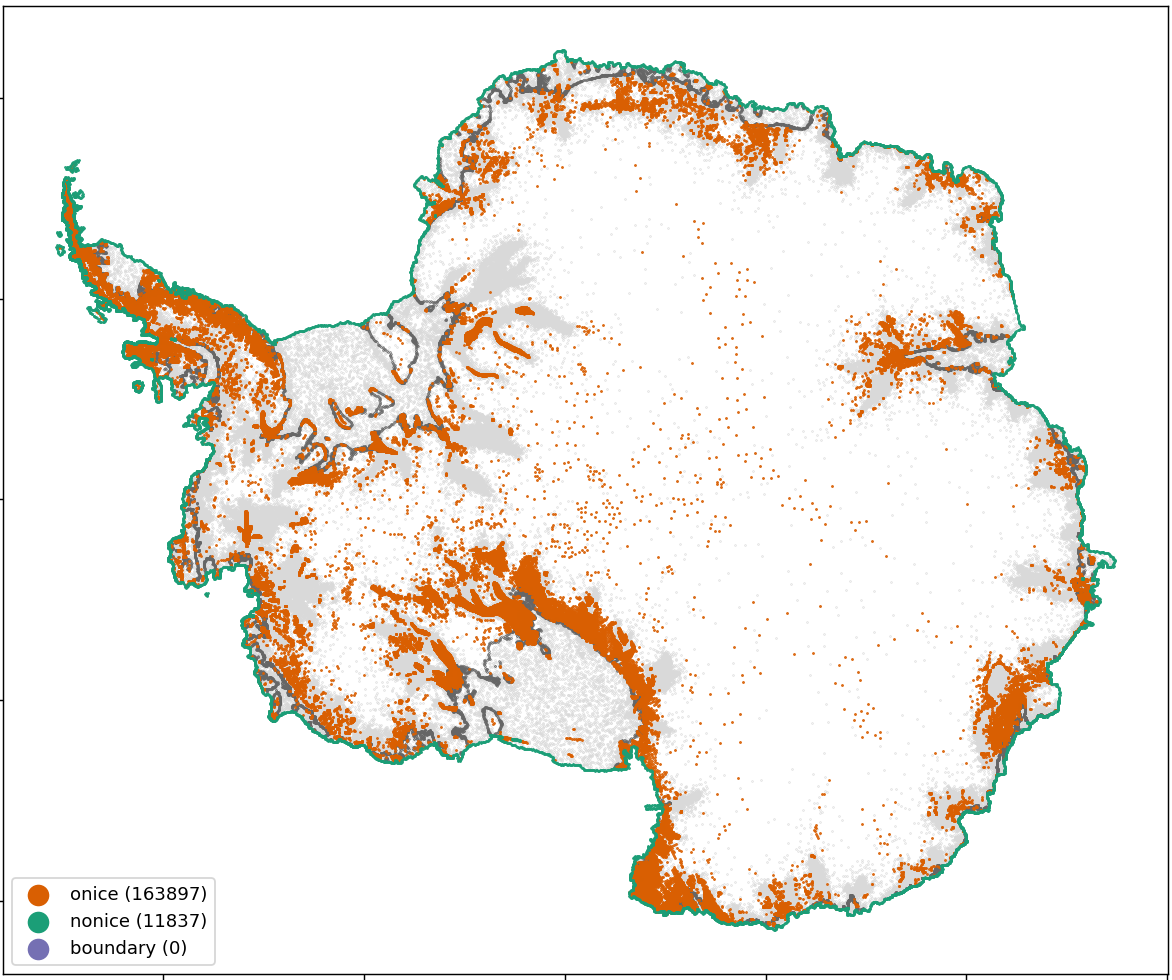
\includegraphics[width=0.92\linewidth]{ho_pins_map.png}
\column{0.6\textwidth}\scriptsize
\begin{tabular}{@{}lrr@{}}
\toprule
\textbf{LARMIP-3 sector} & \textbf{grounded pinned} & \textbf{GL flux pinned}\\
\midrule
3 Ross & 13.8\% & \hl{64\%}\\
1 Weddell & 8.4\% & 20\%\\
2 EAIS & 5.7\% & 7\%\\
5 Peninsula & 22.8\% & 5\%\\
4 Amundsen & 5.0\% & 2\%\\
\bottomrule
\end{tabular}\par\vspace{2mm}
\begin{itemize}
\item 175,734 pinned columns (164k on ice, 12k ice-free) from the Schoof-subdomain fixes
\item Pinned convergent flow $\rightarrow$ runaway $H$: 875 m (2019) $\rightarrow$ 226 km (2220); $<$7 mm SLE
\item Unpin test, stress balance only: max speed 4.2 km/yr (pins) vs $7\times10^5$ (on-ice released) vs $7\times10^8$ m/yr (all)
\item Pins stay. A pin-free HO needs a new friction inversion
\end{itemize}
\end{columns}
\note{Pins: thin ice H <= 100 m, C at the lower bound (50), and ice_levelset >= 0 vertices in the Schoof subdomain, ais_0.1.py ~1596-1653. Spike vertices mostly on ice-free or floating vertices, so the ISMIP VAF barely sees them.}
\end{frame}

% ============================================================ ops
\nosource
\begin{frame}{Operations: two SIGBUS stalls, now caught in minutes}
\framesubtitle{Compute and robustness}
\vspace{2mm}\small
\begin{columns}[T]
\column{0.48\textwidth}
{\serif\large\bfseries\color{navy}What went wrong}
\begin{itemize}
\item Two ctrl inner solves killed by SIGBUS (30, 31 Oct), different nodes, not reproducible
\item Drivers waited blindly for the lock: 18 h and 43 h lost
\item One transient HDF read error on a 58 GB checkpoint
\end{itemize}
\column{0.48\textwidth}
{\serif\large\bfseries\color{navy}What changed}
\begin{itemize}
\item Watched solve ported to HO: polls lock + PBS footer, one retry
\item 7+ HO chunks clean since; $\sim$13 h per 10-yr chunk
\item $\sim$95k SU per HO run to 2300; Q4 allocation 1.35 MSU
\item gdata 56.7 of 100 TiB
\item GPU (hypre BoomerAMG, 1 A100): 1-yr SSA transient 1.5$\times$ faster, 1.9$\times$ fewer SU than 48-core MUMPS
\end{itemize}
\end{columns}
\end{frame}

% ============================================================ decisions
{\setbeamercolor{background canvas}{bg=paper2}
\begin{frame}{What we need to decide}
\framesubtitle{Next}
\vspace{2mm}\small
\renewcommand{\arraystretch}{1.35}
\begin{tabular}{@{}p{0.3\linewidth}p{0.63\linewidth}@{}}
\toprule
{\bfseries\color{navy}Paper scope} & GMD model description + evaluation: SSA projections, HO as check, LARMIP diagnosis, collapse\\
{\bfseries\color{navy}More collapse runs} & which scenario/GCM next (e.g. ssp585 high melt, MRI ssp585, ssp126)\\
{\bfseries\color{navy}Collapse residue} & keep 1e-2 or rerun at 1e-3\\
{\bfseries\color{navy}HO after 2100} & robustness check only, or invest in a pin-free friction inversion\\
{\bfseries\color{navy}Sensitivity gap} & next test: GL drag, resolution, or HO in Amundsen only\\
{\bfseries\color{navy}Housekeeping} & commit watched-solve + check scripts; ISMIP6 comparison; Zenodo DOI\\
\bottomrule
\end{tabular}
\end{frame}}

\end{document}
